% !TeX spellcheck = en_US
%%
%% sample document for AAMAS'18 conference
%%
%% modified from sample-sigconf.tex
%%
%% see ACM instructions acmguide.pdf
%%
%% AAMAS-specific questions? n.yorke-smith@tudelft.nl
%%

\documentclass[sigconf]{aamas}  % do not change this line!

%% your usepackages here, for example:
\usepackage{booktabs}
\usepackage{graphicx}
\usepackage[rflt]{floatflt}
\usepackage{subcaption} 
\usepackage{frame, caption}
\usepackage{amsmath}
\usepackage{mathrsfs}
\usepackage{array}

\newcommand{\argmax}{\operatornamewithlimits{arg\,max}}

%% do not change the following lines
\setcopyright{ifaamas}  % do not change this line!
\acmDOI{doi}  % do not change this line!
\acmISBN{}  % do not change this line!
\acmConference[AAMAS'18]{Proc.\@ of the 17th International Conference on Autonomous Agents and Multiagent Systems (AAMAS 2018), M.~Dastani, G.~Sukthankar, E.~Andre, S.~Koenig (eds.)}{July 2018}{Stockholm, Sweden}  % do not change this line!
\acmYear{2018}  % do not change this line!
\copyrightyear{2018}  % do not change this line!
\acmPrice{}  % do not change this line!

%% the rest of your preamble here


%%%%%%%%%%%%%%%%%%%%%%%%%%%%%%%%%%%%%%%%%%%%%%%%%%%%%%%%%%%%%%%%%%%%%%%%%%%%%%%%%%%%%%%%%%%%%%%%%%%%%%%%%

%%%%%%%%%%%%%%%%%%%%%%%%%%%%%%%%%%%%%%%%%%%%%%%%%%%%%%%%%%%%%%%%%%%%%%%%%%%%%%%%%%%%%%%%%%%%%%%%%%%%%%%%%

\begin{document}
	
	\title{I've got the power's value! A computational model to evaluate the interlocutor's behaviors in collaborative negotiation}  % put your title here!

	\subtitle{Socially Interactive Agents Track}

	
	% AAMAS: submissions are anonymous for most tracks
	\author{Paper \#32}  % put your paper number here!
	

	%
	%\author{Ben Trovato}
	%\authornote{Dr.~Trovato insisted his name be first.}
	%\orcid{1234-5678-9012}
	%\affiliation{%
	%  \institution{Institute for Clarity in Documentation}
	%  \streetaddress{P.O. Box 1212}
	%  \city{Dublin} 
	%  \state{Ohio} 
	%  \postcode{43017-6221}
	%}
	%\email{trovato@corporation.com}
	%
	%\author{G.K.M. Tobin}
	%\authornote{The secretary disavows any knowledge of this author's actions.}
	%\affiliation{%
	%  \institution{Institute for Clarity in Documentation}
	%  \streetaddress{P.O. Box 1212}
	%  \city{Dublin} 
	%  \state{Ohio} 
	%  \postcode{43017-6221}
	%}
	%\email{webmaster@marysville-ohio.com}
	%
	%\author{Lars Th{\o}rv{\"a}ld}
	%\authornote{This author is the
	%  one who did all the really hard work.}
	%\affiliation{%
	%  \institution{The Th{\o}rv{\"a}ld Group}
	%  \streetaddress{1 Th{\o}rv{\"a}ld Circle}
	%  \city{Hekla} 
	%  \country{Iceland}}
	%\email{larst@affiliation.org}
	%
	%\author{Valerie B\'eranger}
	%\affiliation{%
	%  \institution{Inria Paris-Rocquencourt}
	%  \city{Rocquencourt}
	%  \country{France}
	%}
	%\author{Aparna Patel} 
	%\affiliation{%
	% \institution{Rajiv Gandhi University}
	% \streetaddress{Rono-Hills}
	% \city{Doimukh} 
	% \state{Arunachal Pradesh}
	% \country{India}}
	%\author{Huifen Chan}
	%\affiliation{%
	%  \institution{Tsinghua University}
	%  \streetaddress{30 Shuangqing Rd}
	%  \city{Haidian Qu} 
	%  \state{Beijing Shi}
	%  \country{China}
	%}
	%
	%\author{Charles Palmer}
	%\affiliation{%
	%  \institution{Palmer Research Laboratories}
	%  \streetaddress{8600 Datapoint Drive}
	%  \city{San Antonio}
	%  \state{Texas} 
	%  \postcode{78229}}
	%\email{cpalmer@prl.com}
	%
	%\author{John Smith}
	%\affiliation{\institution{The Th{\o}rv{\"a}ld Group}}
	%\email{jsmith@affiliation.org}
	%
	%\author{Julius P.~Kumquat}
	%\affiliation{\institution{The Kumquat Consortium}}
	%\email{jpkumquat@consortium.net}
	%
	%% The example's default list of authors is too long for headers
	%\renewcommand{\shortauthors}{B. Trovato et al.}
	
	
	\begin{abstract}  % put your abstract here!
		
	
		
	\end{abstract}
	

	\keywords{Dominance; Reasoning about other; Theory of mind}  % put your semicolon-separated keywords here!
	
	\maketitle

	
	\section{Introduction}
	
	Negotiation is a common task in daily life. People negotiate not only in professional situations (\emph{e.g.} for a salary increase or a promotion) but also in more simple situations such as choosing the holiday's destination. In the last decade, a variety of conversational agents which negotiate with people  have been created \cite{pynadath2013you,gratch2016misrepresentation,klatt2011negotiations}. Theses agents are designed with a growing number of decisional abilities, including multi-party and multi-issues negotiation capabilities.
	
	However, negotiation is a multifaceted process which also involves social interaction, affects as well as personal preferences and opinions  \cite{bro2010affective}. Several research considered the role social behavior in the negotiation process. For instance, \cite{traum2008multi} defined a negotiator agent capable of deploying several strategies, constructed based on multiple social factors such as trust and commitment. 
	\cite{de2011effect} studied how the expression of emotions such as anger and happiness affects the strategies of negotiators, and by consequences the outcomes of the negotiation. 
	%In the same vein, \cite{kraus1995designing} developed an agent that behaves according to different personalities and has a learning mechanism to learn the personality of its opponents.
	
	One key element in the social aspect is the \emph{interpersonal relation} between the agent and a human user. 
	%We focus in the following paper on the relation of dominance. 
	Indeed, researches in social psychology demonstrated that the relation of dominance affects the way that the negotiation process is perceived \cite{van2006power}. Negotiating parties often differ in terms of dominance and this difference exerts an important influence on the behavior of participants. Negotiators build different negotiation strategies depending on their relative dominance which directly influences the outcomes of the negotiation. 
	More precisely, Tidens \cite{tiedens2003power} showed that dominance complementarity (\emph{i.e.} one negotiator exhibits dominant behaviors while the other one responds with submissive ones) leads the negotiators to reach mutually beneficial outcomes and increases their reciprocal likings. \cite{wiltermuth2015benefits,tiedens2003power}.
	
	In addition, dominance is represented as a dyadic variable in which control attempts by one individual are accepted by the partner, which means if one individual expresses behaviors of high power, the interactional partner will adapt with a low power behavior \cite{burgoon1998nature}. 
	
	
	In order to build an agent which considers its relation of dominance with a human interlocutor, the agent has to be able to express and understand behaviors related to power. To this aim, we presented in a previous work \cite{ouali2017computational} a computational model of negotiation in which an agent is allowed to express its behavior of power through its strategy of negotiation. First, we defined principles of negotiation based on power inspired from social psychology \cite{de1995impact,van2004interpersonal,van2006power,magee2007power}. Second, we presented a computational model of collaborative negotiation, in which the decisional model takes into account those principles of power to build the agent's negotiation strategy. 
	Finally, we presented an experimental study showing that external judges were able to perceive behaviors of power expressed by an artificial agent in the context of agent/agent negotiation.
	
	
	Taking this computational model as a point of departure, we propose, to create a negotiator agent able to simulate a \emph{complementary relation of dominance} with its interlocutor. To this aim, the agent has to understand the behaviors of power expressed by the interlocutor so as to adapt a complementary behavior.

	We propose to implement this complementarity using mechanisms inspired from theory of mind. More specifically, we use mechanisms of \emph{simulation theory} \emph{ST} which suggests that humans, have the ability to project oneself in the other person's shoes \cite{shanton2010simulation}. Therefore, we can simulate his or her mental activity with our own capacities for practical reasoning. 
	Thus, we can mimic the mental state of our interactional partner \cite{harbers2009modeling}.
	
	We present in this paper a model of ToM with a \emph{ST} approach, in which the agent uses its model of decision based on power in order to reason about its interlocutor's behavior and guess his/her behaviors of power. By consequence, the agent can adapt its behaviors to the behavior guessed in order to create a complementary relation of dominance as illustrated in figure \ref{fig:schema-general}.
	
	
	 
	
	
	\begin{figure*}
		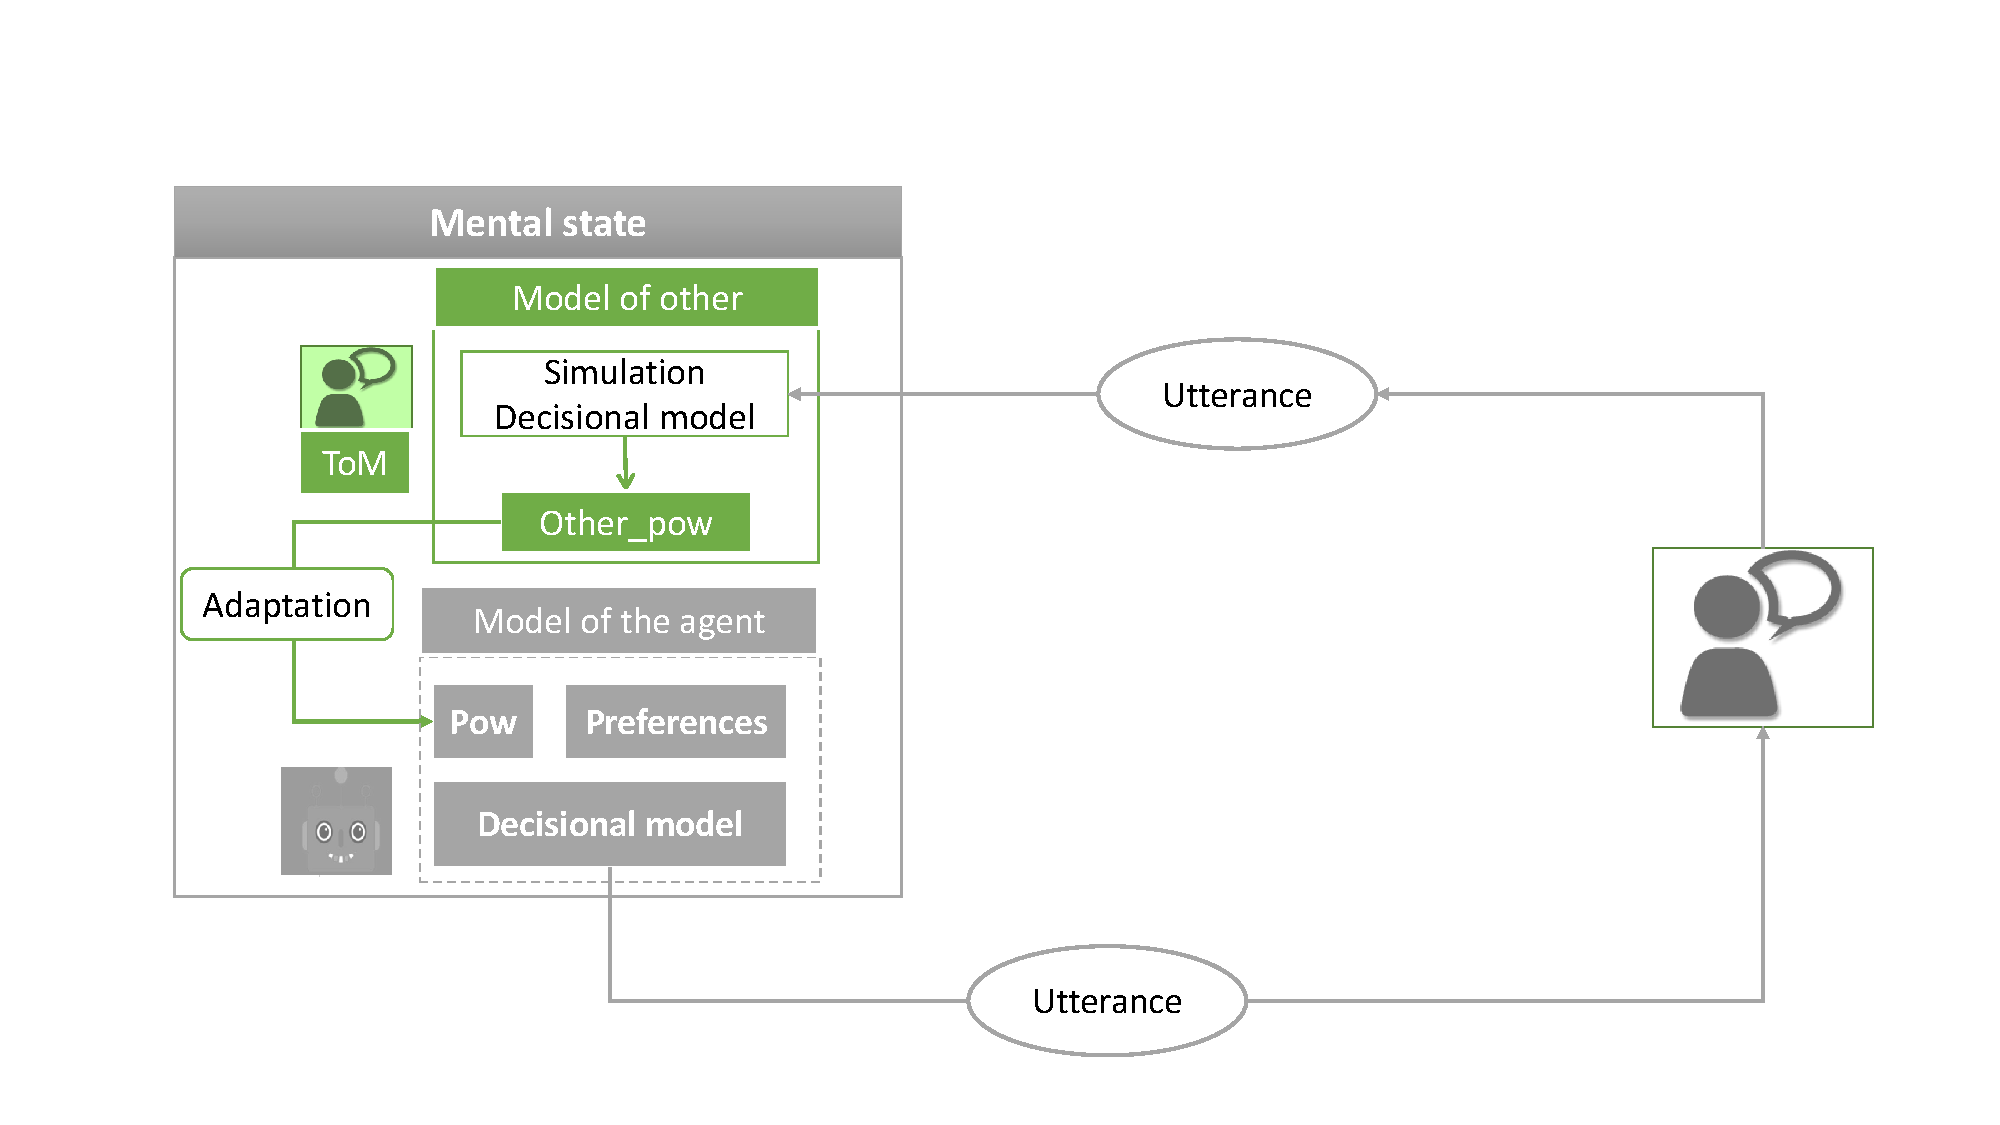
\includegraphics[width=0.65\linewidth, height= 0.25\textheight]{figs/model_tom.pdf}
		\caption{Model of collaborative negotiation with a model of other} 
		\label{fig:schema-general}
	\end{figure*} 


	\section{Negotiator agent with ToM}
		Present mental state of the agent (domain, communication) 
		
		Decision during the negotiation is built to take into account the preferences of the agent as well as his power. 
		Conclusion 1: in order to guess the user power, based on its behaviors (produced utterances) the agent has to make hypotheses about its mental state (preferences, power). Since, our aim is to guess the power, we propose a model in which the agent has a partial representation of preferences. 
		
		We propose an adaptation of the agent decision model to handle partial knowledge of preferences. 
		
	\section{Conclusion}

	
	%%%%%%%%%%%%%%%%%%%%%%%%%%%%%%%%%%%%%%%%%%%%%%%%%%%%%%%%%%%%%%%%%%%%%%%%%%%%%%%%%%%%%%%%%%%%%%%%%%%%%%%%%
	%% bibliography: see CFP for number of permitted pages
	
	\bibliographystyle{ACM-Reference-Format}  % do not change this line!
	\bibliography{bibliography}  % put name of your .bib file here
	
\end{document}